% 	This template is  MIT licensed.

% 	Basic file to demonstrate the usage of this LaTeX template.
% 	You can build your own paper/thesis on top of this file.
% 	Simply adjust the document class and all metadata and start working.
%
\documentclass[
	language=english, % set to english or german
	type=master, % set to bachelor, master or seminar
]{isthesis}

\usepackage[utf8]{vntex}

% custom package
\usepackage{eurosym}
\usepackage{makecell}
\usepackage{hyperref}
\usepackage[utf8]{inputenc}
\usepackage{tabto} 
\usepackage{longtable}
\usepackage{algorithm} 
\usepackage{algpseudocode}
\usepackage{biblatex} %Imports biblatex package
% \usepackage{multirow}
% \usepackage{floatrow}

% Graphics rendering using TikZ
% See: https://en.wikibooks.org/wiki/LaTeX/PGF/TikZ
\usepackage{tikz}
\usepackage{xcolor}
\definecolor{light-gray}{gray}{0.95}
\newcommand{\code}[1]{\colorbox{light-gray}{\texttt{#1}}}
% Include required TikZ libraries here, some exemplary libraries are pre-included
\usetikzlibrary{calc}
\usetikzlibrary{matrix}
\usetikzlibrary{positioning}
\usetikzlibrary{shapes.geometric}

\usepackage{amsthm}
% \usepackage{ntheorem}
\newtheoremstyle{theoremst}% name of the style to be used
  {\topsep}% measure of space to leave above the theorem. E.g.: 3pt
  {\topsep}% measure of space to leave below the theorem. E.g.: 3pt
  {\normalfont}% name of font to use in the body of the theorem
  {0pt}% measure of space to indent
  {\bfseries}% name of head font
  {:}% punctuation between head and body
  { }% space after theorem head; " " = normal interword space
  {\thmname{#1}\thmnumber{ #2}\textnormal{\thmnote{ (#3)}}}

\newtheoremstyle{examplest}% name of the style to be used
  {\topsep}% measure of space to leave above the theorem. E.g.: 3pt
  {\topsep}% measure of space to leave below the theorem. E.g.: 3pt
  {\normalfont}% name of font to use in the body of the theorem
  {0pt}% measure of space to indent
  {\bfseries}% name of head font
  {\\}% punctuation between head and body
  { }% space after theorem head; " " = normal interword space
  {\thmname{#1}\thmnumber{ #2}\textnormal{\thmnote{ (#3)}}}


% \theorembodyfont{\normalfont}
% \theoremseparator{:}
\theoremstyle{theoremst}
\newtheorem{definition}{Định nghĩa}[section]
\newtheorem{theorem}{Định lý}[section]
\newtheorem{proposition}{Khẳng định}[section]

% \theoremstyle{break}
% \theorembodyfont{\normalfont}
\theoremstyle{examplest}
\newtheorem{remark}{Nhận xét}[section]
\newtheorem{example}{Ví dụ}[section]

% \theoremstyle{remark}
% \newtheorem*{remark}{Remark}

%Add your library here
\addbibresource{refs.bib}

% Import acronyms
% \newacronym[longplural={<long plural>}, shortplural={<short plural>}]{<label>}{<short>}{<long>}
% 	label = is the unique identifier and sort key for the acronym, can be the same as <short>
%	short = is the abbreviation or acronym
%	short plural (optional) = is the plural of the abbreviation or acronym
%	long = is the long form of the acronym, this will appear in the list of abbreviations
%	long plural (optional) = is the long plural form of the abbreviation or acronym

\newacronym[shortplural={KMUen}, longplural={Kleine und Mittlere Unternehmen}]{kmu}{KMU}{Kleines und Mittleres Unternehmen}
\newacronym{CD}{CD}{Corporate Design}
\newacronym{SQL}{SQL}{Structured Query Language}
\newacronym{FAU}{FAU}{Khoa Toán cơ tin}
\newacronym{BPM}{BPM}{Business Process Management}
\newacronym{npm}{NPM}{Node Package Manager}
\newacronym{diss}{DISS}{Digital Industrial Service System}

% Import symbols
% Syntax: <Symbol> <Label> <Name>
% The symbols are sorted by their labels
\addsymboltolist{$\Pi$}{Pi}{Projection}
\addsymboltolist{$\Join$}{Join}{Natural Join}
\addsymboltolist{$\sigma$}{Selection}{Selection}


% Import custom commands
% If you want to define custom commands, please do so here

% Import custom code block
% define listing code
\definecolor{codegreen}{rgb}{0,0.6,0}
\definecolor{codegray}{rgb}{0.5,0.5,0.5}
\definecolor{codepurple}{rgb}{0.58,0,0.82}
\definecolor{backcolour}{rgb}{0.95,0.95,0.92}

\lstdefinestyle{code}{
    backgroundcolor=\color{backcolour},   
    commentstyle=\color{codegreen},
    keywordstyle=\color{magenta},
    numberstyle=\tiny\color{codegray},
    stringstyle=\color{codepurple},
    basicstyle=\ttfamily\footnotesize,
    breakatwhitespace=false,         
    breaklines=true,                 
    captionpos=b,                    
    keepspaces=true,                 
    numbers=left,
    firstnumber=1,
    stepnumber=1,                    
    numbersep=5pt,                  
    showspaces=false,                
    showstringspaces=false,
    showtabs=false,                  
    tabsize=2,
    framesep=10pt,
    xleftmargin=10pt,
    xrightmargin=10pt,
    framexleftmargin=16pt,
    framextopmargin=2pt,
    framexbottommargin=2pt, 
    frame=tb, framerule=0pt,
}

\lstdefinestyle{algo}{
    backgroundcolor=\color{backcolour},   
    commentstyle=\color{codegreen},
    keywordstyle=\color{magenta},
    numberstyle=\tiny\color{codegray},
    stringstyle=\color{codepurple},
    basicstyle=\ttfamily\footnotesize\small\linespread{0.8},
    breakatwhitespace=false,         
    breaklines=true,                 
    captionpos=b,                    
    keepspaces=true,                 
    numbers=none,
    firstnumber=1,
    stepnumber=1,                    
    numbersep=5pt,                  
    showspaces=false,                
    showstringspaces=false,
    showtabs=false,                  
    tabsize=2,
    framesep=10pt,
    xleftmargin=10pt,
    xrightmargin=10pt,
    framexleftmargin=16pt,
    framextopmargin=2pt,
    framexbottommargin=2pt, 
    frame=tb, framerule=0pt,
    mathescape=true
}

\lstset{style=code}

% Document meta information
\isthesis{
    title={LUẬN VĂN THẠC SĨ},
    sub-title={Phương pháp tìm kiếm lân cận rộng thích ứng \\  
    cho bài toán định tuyến xe},
    author-name={Nguyễn Mạnh Linh}, 
    % Separate multiple authors with commas
    % author-email={linhnguyen.code@gmail.com},
    % author-matriculation={MATRICULATION NUMBER},
    % author-phone={+49 XXXXXXXXX}, % Use international numbers format
    % author-address={STREET},
    % author-zip={ZIP},
    % author-city={CITY},
    principal-supervisor={TS. Hoàng Nam Dũng}, % This must be a professor
    % associate-supervisor={SUPERVISOR}, % This is your main supervisor, i.e., a post doc or doctoral student
    tutor-supervisor={}, % If required, define an additional supervisor resp. tutor here
    group-institute={Trường Đại học Khoa học Tự nhiên},
    % group={Image Data Exploration and Analysis (IDEA) Lab},
    % studies={M.Sc. International Information Systems}, %your field of studies, i.e. Wirtschaftsinformatik or International Information Systems
    %
    %associate-group={}, % When the thesis is done in cooperation with another chair, add it here
    %associate-group-institute={}, % add cooperating institute or university here
    seminar={SEMINAR}, % The title of your seminar
    submission-date={2023-11-01}, % The date you handed in your document: Format yyyy-mm-dd
    primary-logo={assets/hus.png}, % Uses the FAU logo by default
    %primary-logo-height={}, % Uses 16mm as default height
    %secondary-logo={}, % Logo of the secondary institution (cooperating chair/university), USES Faculty logo by default
    %secondary-logo-height={} % Uses 16mm as default height
}


\begin{document}
    % Title page
    \newcounter{savepage}
    \maketitle

	% Quote
    % You can put an optional quote page in front of your content
    %   \quotepage[author={Arthur C. Clarke}]{
    %   	        Any sufficiently advanced technology is indistinguishable from magic.
    %   }
    
    % Table of contents
    \tableofcontents

    % \begin{abstract}
   Trong luận văn này, tác giả nghiên cứu mô hình toán học cho lớp các bài toán định tuyến xe (\textit{Vehicle Routing Problem} - VRP). Các thuật toán liên quan được giới thiệu và phân loại xuyên suốt lịch sử hơn $60$ năm phát triển của VRP. Thuật toán \textit{Tìm kiếm lân cận rộng thích ứng} (\textit{Adaptive Large Neighborhood Search}) được sử dụng để giải bài toán \textit{Định tuyến xe với ràng buộc khung thời gian} (\textit{Vehicle Routing Problem with Time Window - VRPTW}). Hai thuật toán hủy mới được tác giả phát triển giúp giảm nhanh số xe sử dụng và tăng hiệu năng khi xóa yêu cầu. Thêm vào đó, tác giả đề xuất một hiệu chỉnh cho ALNS được gọi là B-ALNS (\textit{Boosted - Adaptive Large Neighborhood Search}). Các thuật toán được đánh giá trên các tập dữ liệu với số lượng yêu cầu từ nhỏ ($100$ yêu cầu) tới rất lớn ($1000$ yêu cầu). B-ALNS được chỉ ra có hiệu năng vượt trội so với ALNS (lên tới hơn $30\%$) và tiết kiệm tới $75\%$ tài nguyên tính toán cho một số cấu hình trong khoảng thời gian nhất định. Ngoài ra, tác giả đưa ra gợi ý áp dụng ALNS, B-ALNS cho các tình huống thực tế với mục đích khác nhau.
\end{abstract} 

    \chapter{Mở đầu}
Từ xưa tới nay, giao vận luôn là một trong những ngành đóng vai trò quan trọng trong nền kinh tế. Nó đóng vai trò là một cầu nối giữa các đơn vị sản xuất và người tiêu dùng. Nó cũng là một trong những ngành có ảnh hưởng lớn đến sự phát triển của một quốc gia. 

Từ những thập niên 90 của thế kỉ trước, thời kì bùng nổ của internet đã thúc đẩy một hình thức bán hàng hoàn toàn mới, đó là bán hàng trực tuyến. Hàng loạt các sàn thương mại điện tử lớn ra đời, có thể kể đến như Amazon (Mỹ - 1994), Alibaba (Trung Quốc - 1999), Rakuten (Nhật Bản - 1997). Ngày nay các sàn thương mại điện tử này trở thành những công ty hàng đầu thế giới không chỉ ở lĩnh vực bán hàng mà là cả công nghệ. Việc phát triển vũ bão của các sàn thương mại điện tử dẫn đến số lượng hàng hóa được tiêu thụ trên toàn cầu tăng lên một cách đáng kinh ngạc so với bán hàng truyền thống. Logistic và quản lý chuỗi cung ứng là một trong những xương sống của thương mại điện tử cùng với \textit{nền tảng công nghệ}, \textit{nền tảng thanh toán} hay \textit{chăm sóc khách hàng}... Để quản lý, giao vận số lượng đơn hàng lớn như vậy tới tay khách hàng, cách thức làm việc trong ngành logistic cũng phải thay đổi rất nhiều, áp dụng những công nghệ hiện đại hơn cách làm truyền thống.


    % \begin{abstract}
	%     % Add your abstract here:
        
	% 	% \lipsum[1]
	% \end{abstract}

    % List of figures (if you have figures)
    % \listoffigures

    % List of tables (if you have tables)
    % \listoftables
    
    % List of listings (if you have listings)
	% \lstlistoflistings

    % List of abbreviations (if you use acronyms)
    %\listofabbreviations

    % List of symbols (if you use symbols)
    %\listofsymbols
	
	% Abstract
	%
	% Comment out this part, if you don't require an abstract

	
	% storing the last pagenumber
    \setcounter{savepage}{\value{page}}
    
    
    % Content
    \begin{content}
        % Add your content files:
        \chapter{Định nghĩa và một số kí hiệu}
Trong chương này, chúng ta sẽ đưa ra định nghĩa chính tắc cho lớp các bài toán định tuyến xe. Các định nghĩa này được xây dựng theo ngôn ngữ của lý thuyết đồ thị được đưa ra bởi Toth (2002) \cite{toth2002vehicle}. 

Các bài toán được mô tả thuộc lớp VRP (\textit{vehicle routing problem}) bao gồm \textit{định tuyến xe với ràng buộc tải trọng} - CVRP (\textit{capacited VRP}), \textit{định tuyến xe với ràng buộc khung thời gian} - VRPTW (\textit{VRP with time windows}), \textit{định tuyến xe với lấy và giao hàng} - VRPPD (\textit{VRP with pickup and delivery}).

\begin{figure}[H] % places figure environment here   
  \centering % Centers Graphic
  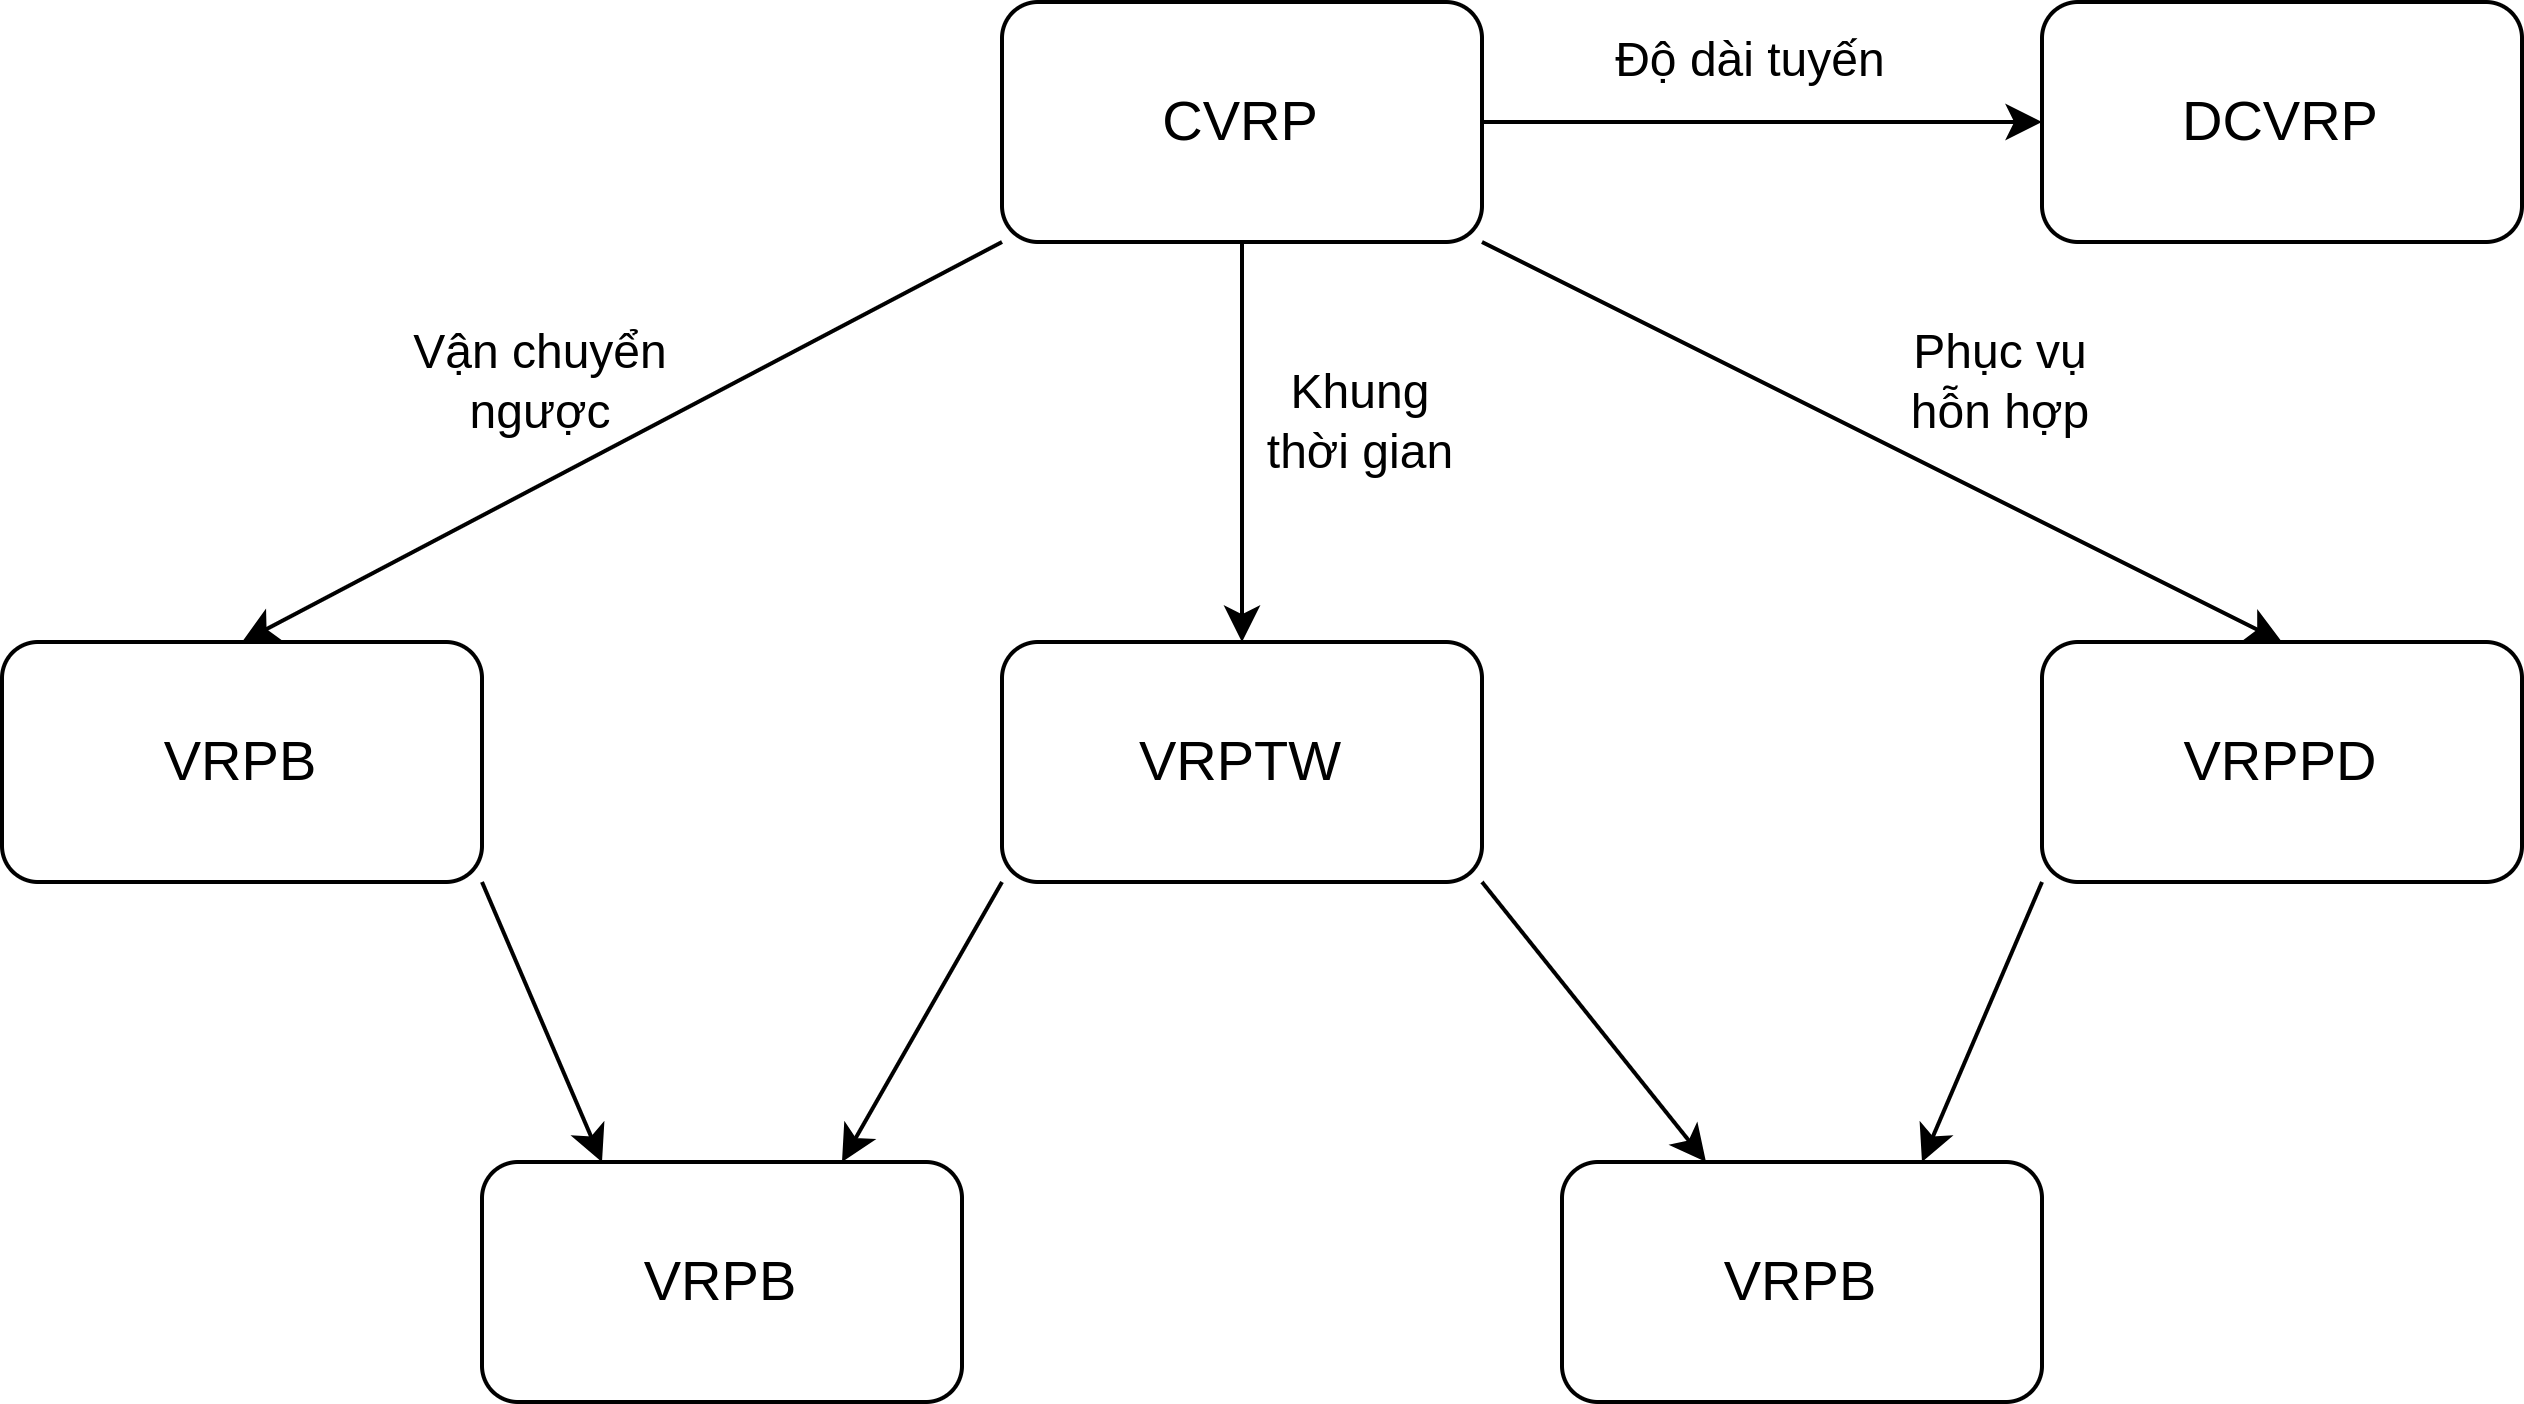
\includegraphics[width=0.8\textwidth]{figures/vrp.png} 
  \caption{Các bài toán, biến thể của VRP} % Creates caption underneath graph
  \label{fig:fg_01}
\end{figure}

\section{CVRP}

Trước hết ta xem xét mô hình cho bài toán \textit{nguyên bản}: \textit{bài toán định tuyến xe với ràng buộc tải trọng}. Một cách tự nhiên, tại sao không phải là VRP (không ràng buộc)? Bạn sẽ thấy rằng nếu không có bất kì ràng buộc nào thì một xe có thể phục vụ tất cả các yêu cầu và bài toán VRP sẽ suy biến về TSP (\textit{travelling salesman problem}). Ít nhất ràng buộc về tải trọng là thực tế và giữ cho mỗi xe chỉ phục vụ được một số yêu cầu nhất định (trong trường hợp số yêu cầu không quá nhỏ cũng như tải trọng của xe là quá lớn). 


Gọi $G=(V,A)$ là một độ thị đầy đủ với $V=\{ 0, ..., n \}$ là tập nút và $A$ là tập các cung. Các nút $i=1,...,n$ đại diện cho các yêu cầu hay khách hàng cần phục vụ, nút $0$ là kho hàng. 

Một số không âm được gọi là chi phí $c_{ij}$ đại diện cho mỗi cung $(i,j) \in A$. Nói cách khác $c_{ij}$ là  chi phí cần bỏ ra để di chuyển từ nút $i$ tới nút $j$. Trong bài toán này và hầu hết các bài toán định tuyến ta không định nghĩa cạnh $(i,i)$ nên có thể gán $c_{ii} = \infty$ với $i \in V$.

Nếu đồ thị là có hướng thì ma trận chi phí $c$ là bất đối xứng, khi đó ta có bài toán CVRP bất đối xứng ACVRP (\textit{asymetric CVRP}). Ngược lại nếu $c_{ij} = c_{ji}$ với mọi $(i,j) \in A$ ta có bài toán CVRP đối xứng SCVRP (\textit{symetric CVRP}) và các cung của $A$ được thay thế bằng tập cách cạnh vô hướng $E$. Với một cạnh $e \in E$, ta định nghĩa $\alpha(e)$ và $\beta(e)$ là nút bắt đầu và kết thúc của cạnh. 

Đồ thị $G$ phải là đồ thị kết nối mạnh và nhìn chung ta giả thiết đồ thị $G$ là đầy đủ. Với một nút $i$, gọi $\Delta^+(i)$ là tập ra của $i$ (\textit{forward star}), được định nghĩa là tập các nút $j$ mà cung $(i,j) \in A$, nói cách khác đây là tập các nút có thể tiếp cận trực tiếp từ nút $i$. Tương tự như vậy, $\Delta^-{i}$ là tập vào của $i$ (\textit{backward star}), được định nghĩa là tập các nút $j$ mà cung $(j,i) \in A$ hay là tập các nút tiếp cận trực tiếp tới nút $i$. Với một tập nút con $S \subseteq V$, gọi $\delta(S)$ là tập các cạnh $e \in E$ chỉ có một hoặc cả hai đầu mút thuộc $S$. Để thuận tiện, khi xét một nút $i \in V$, ta viết $\delta(i)$ thay cho $\delta(\{i\})$.

Trong hầu hết các bài toán thực tế, ma trận chi phí thỏa mãn bất đẳng thức tam giác 
\begin{equation}
    c_{ij} + c_{jk} \geq c_{ik} \quad \forall i,j,k \in V
\end{equation}
Nói cách khác việc đi trực tiếp từ nút $i$ tới nút $j$ luôn tốn ít chi phí hơn là đi gián tiếp. Với nhiều thuật toán, bất đẳng thức tam giác là điều kiện cần, điều này có thể được đảm bảo bằng cách thêm một đại lượng dương lớn (hợp lý) vào chi phí của mỗi cung. Ta chú ý thêm rằng nếu chi phí của mỗi cung thuộc đồ thị bằng với chi phí của đường đi ngắn nhất giữa hai đầu mút của cung thì mà trận chi phí thỏa mãn bất đẳng thức tam giác.

Trong nhiều trường hợp, tập các nút nằm trên một mặt phẳng, vị trí của chúng được cho bởi tọa độ và chi phí $c_{ij}$ của mỗi cung $(i,j) \in A$ là khoảng cách Euclide giữa hai điểm ứng với nút $i$ và $j$. Khi đó, ma trận chi phí là đối xứng và thỏa mãn bất đẳng thức tam giác. Bài toán này được gọi là \textit{Euclidian} SCVRP.

Mỗi khách hàng $i$ có một nhu cầu (về tải trọng) là $d_i$ và nhu cầu của kho $d_0=0$. Với một tập nút $S \subseteq V$, ta kí hiệu $d(S) = \sum_{i \in S} d_i$ là tổng nhu cầu của tập.

Một tập hợp $K$ đại diện cho các xe, mỗi xe có tải trọng $C$ và sẵn sàng ở kho. Ta giả thiết $d_i \leq C$ với mỗi $i=1,...,n$. Giả thiết này là cần thiết để  mỗi khách hàng đều được phục vụ. Mỗi xe phục vụ nhiều nhất một tuyến và ta giả thiết $K$ không nhỏ hơn $K_{min}$ với $K_{min}$ là số xe ít nhất cần để phục vụ toàn bộ khách hàng. 

Với một tập $S \subseteq V \setminus \{0\}$, ta gọi $r(S)$ là số xe ít nhất để phục vụ toàn bộ khách hàng thuộc tập $S$. Chú ý rằng $r(V \setminus \{0\}) = K_{min}$.

CVRP yêu cầu tìm một tập chính xác $K$ các chu trình đơn (mỗi chu trình ứng với một tuyến đường) với tổng chi phí của tất cả các cung thuộc các chu trình này là nhỏ nhất. Lời giải phải thỏa mãn các ràng buộc sau:
\begin{itemize}
  \item[] (i) Mỗi chu trình đều đi qua nút ứng với kho hàng
  \item[] (ii) Mỗi nút ứng với một khách hàng được đi qua bởi đúng một chu trình 
  \item[] (iii) Tổng nhu cầu của các khách hàng trong mỗi chu trình không được vượt quá tải trọng của xe.
\end{itemize}

\section{CVRPTW}
Bài toán định tuyến xe với ràng buộc thời gian - VRPTW (\textit{VRP with time windows}) là một mở rộng của CVRP. Trong đó ngoài ràng buộc về tải trọng cho mỗi xe, mỗi khách hàng $i$ bị ràng buộc bởi một khoảng thời gian $[a_i, b_i]$ được gọi là khung thời gian hay cửa sổ thơi gian (\textit{time window}). Thời gian phục vụ khách hàng $i$ là $s_i$. Thời gian di chuyển từ nút $i$ tới nút $j$ là $t_{ij}$ với mỗi cung $(i,j) \in A$ hay $t_e$ với $e \in E$. Ngoài ra nếu xe đến nút $i$ sớm thì phải chờ đến thời gian $a_i$ mới được phục vụ. Nếu xe đến nút $i$ muộn hơn thì khách hàng sẽ không được phục vụ.

Thường thì ma trận chi phí và ma trận thời gian di chuyển là như nhau, hơn nữa các xe được giả thiết đều xuất phát từ kho tại thời điểm $0$. Ràng buộc thời gian dẫn tới mỗi tuyến đường là có hướng (có thứ tự đi đến các nút) ngay cả khi ma trận chi phí là đối xứng. Chính vì thế, VRPTW thường được mô tả như một bài toán bất đối xứng.

VRPTW yêu cầu tìm một tập chính xác $K$ chu trình đơn với tổng chi phí là nhỏ nhất, thỏa mãn các ràng buộc sau đây:
\begin{itemize}
  \item[] (i) Mỗi chu trình đều đi qua nút ứng với kho hàng
  \item[] (ii) Mỗi nút ứng với một khách hàng được đi qua bởi đúng một chu trình
  \item[] (iii) Tổng nhu cầu của các khách hàng trong mỗi chu trình không được vượt quá tải trọng của xe
  \item[] (iv) Với mỗi khách hàng $i$, thời gian bắt đầu phục vụ phải nằm trong khung thời gian $[a_i, b_i]$ và xe ngừng phục vụ sau khoảng thời gian $s_i$
\end{itemize}

VRPTW là bài toán NP-khó, nó là trường hợp tổng quát của CVRP. Nếu ta đặt $a_i=0$ và $b_i=\infty$ với $i \in V \setminus \{0\}$ thì VRPTW suy biến về CVRP. Ngoài ra ta cũng thu được biến thể TSP với ràng buộc thời gian (TSPTW) nếu $C \geq d(V)$ và $K=1$.

\section{VRPPD}
Một biến thể khác nữa của CVRP là bài toán định tuyến xe với lấy và giao hàng (\textit{VRP with pickup and delivery - VRPPD}). Trong đó, mỗi khách hàng $i$ có thêm hai đại lượng đặc trưng nữa là $d_i$ và $p_i$ lần lượt là nhu cầu lấy và giao tại khách hàng $i$. Đôi khi chỉ một đại lượng $d_i = d_i - p_i$ được sử dụng cho mỗi khách hàng $i$ để chỉ lượng nhu cầu chênh lệch giữa việc lấy và giao hàng (có thể là số âm). Với mỗi khách hàng $i$, gọi $O_i$ là nút đại diện cho việc giao hàng và $D_i$ là nút đại diện cho điểm lấy hàng. 

Giả thiết rằng, tại mỗi điểm khách hàng, điểm giao được phục vụ trước điểm lấy. Do đó, tải hiện tại của một xe trướ khi tới điểm đã cho là tải ban đầu trừ đi tổng nhu cầu đã giao cộng với tổng nhu cầu đã lấy.

VRPPD yếu cầu tìm chính xác một tập $K$ các chu trình đơn với tổng chi phí là nhỏ nhất, thỏa mãn các ràng buộc sau đây:

\begin{itemize}
  \item[] (i) Mỗi chu trình đều đi qua nút ứng với kho hàng
  \item[] (ii) Mỗi nút ứng với một khách hàng được đi qua bởi đúng một chu trình
  \item[] (iii) Tải hiện tại của xe trong suốt quá trình phục vụ không âm và không được vượt quá tải trọng của xe
  \item[] (iv) Với mỗi khách hàng $i$, khách hàng $O_i$ khác với kho phải được phục vụ trong cùng một tuyến và trước khách hàng $i$
  \item[] (v) Với mỗi khách hàng $i$, khách hàng $D_i$ khác với kho phải được phụ vụ trong cùng một tuyến và sau khách hàng $i$.
\end{itemize}

VRPPD là trường hợp tổng quát của CVRP. Nếu ta đặt $O_i = D_i = 0$ và $p_i = 0$ cho mọi $i \in V$ thì VRPPD suy biến về CVRP. Hơn nữa nếu đặt $K=1$ thì ta thu được TSP với lấy và giao hàng (\textit{TSP with pickup and delivery - TSPPD}).

        \chapter{Mô hình toán học}
Chương này trình bày biểu diễn toán học cho bài toán VRPTW. Trong luận văn này, tác giả tập trung giải quyết VRPTW, từ đó ta cũng có thể giản ước về CVRP cũng như tổng quát với VRPPD (\textit{VRP with pickup and delevery}) hoặc PDPTW (\textit{pickup and delivery with time window}). Như đã trình bày ở chương trước VRPTW là một mở rộng của CVRP với ràng buộc khung thời gian. Trong đó mỗi khách hàng $i$ được ràng buộc bởi một khung thời gian $[a_i,b_i]$. Xe không được đến $i$ tại thời điểm $t_i > b_i$, ngoài ra nếu đến sớm hơn thởi điểm $a_i$ hay $t_i < a_i$ thì xe cần phải chờ tới thời điểm $a_i$ để phục vụ khách hàng. Thời gian phục vụ của khách hàng $i$ là $s_i$.

VRPTW là bài toán NP-khó, việc tìm lời giải hay nghiệm tối ưu (chính xác) gần như là bất khả thi. Để dễ hình dung, xét bài toán VRP, với số lượng khách hàng $n=100$, và chỉ một xe, số lượng lời giải là $n! \approx 10^{158}$. Nếu ta có số CPU ước tính bằng toàn bộ số nguyên tử trong vũ trụ $n_{CPU} \approx 10^{80}$, thời gian nhỏ nhất là thời gian Plank $t_p \approx 5.39 \times 10^{-44}$. Để kiểm tra toàn bộ lời giải có phải nghiệm tối ưu ta cần thời gian $T \approx 10^{158} \times 5.39 \times 10^{-44} / 10^{80} \approx 5.39 \times 10^{34}$. Để so sánh, tuổi của vũ trụ được ước tính khoảng $4.33 \times 10^{17}$. Nghĩa là ta sẽ mất thời gian lớn gấp cỡ \textit{một trăm triệu tỉ} lần tuổi của cả vũ trụ! \footnote[1]{Slides của Thibaut Vidal (SOICT, Nha Trang 2017)}

\section{Biểu diễn toán học}
Như đã trình bày ở chương trước, VRPTW được định nghĩa trên đồ thị $G = (V, A)$, kho hàng được biểu diễn bởi nút $0$ và $n+1$. Một tuyến thỏa mãn là một đường đi trên đồ thị $G$ bắt đầu từ $0$ và kết thúc ở $n+1$. Nếu kho hàng được biểu diễn chỉ bởi nút $0$ thì tuyến thỏa mãn là một đơn chu trình trên đồ thị $G$ chứ nút $0$. Khung thời gian của nút $0$ và $n+1$ là $[a_0, b_0] = [a_{n+1}, b_{n+1}] = [E, L]$, trong đó $E$ và $L$ lần lượt là thời gian sớm nhất rời kho và thời gian muộn nhất trở về kho. Ngoài ra, thời gian phục vụ và nhu cầu của kho đều được đặt bằng 0, hay $s_0 = s_{n+1} = 0$ và $d_0 = d_{n+1} = 0$. Lời giải chấp nhận được chỉ tồn tại nếu $a_0 = E \leq \min_{i \in V \setminus \{0\}} \{b_i - t_{0i}\}$ và $b_{n+1} = L \geq \min_{i \in V \setminus \{0\}} \{ a_i + s_i + t_{0i} \}$. Chú ý rằng, cung $(i,j) \in A$ có thể được bỏ đi nếu không thỏa mãn ràng buộc thời gian $a_i + s_i + t_{ij} > b_j$ hoặc vi phạm ràng buộc về tải trọng $d_i + d_j > C$. Cuối cùng nếu mục tiêu chính là giảm thiểu số lượng xe thì cung $(0,n+1)$ với $c_{0,n+1} = t_{0,n+1} = 0$ phải được thêm vào $A$.

Tiếp theo, chúng ta trình bày một mô hình toán cho VRPTW với hai biến: biến $x_{ijk}$ (\textit{flow variable}) với $(i,j) \in A, k \in K$ nhận giá trị 1 nếu xe $k$ đi trực tiếp từ nút $i$ tới nút $j$ và 0 nếu ngược lại. Biến $w_{ik}$ với $i \in V, k \in K$ là thời gian bắt đầu phục vụ khách hàng $i$ bởi xe $k$. VRPTW được mô hình một cách chính tắc như sau theo Toth (2002) \cite{toth2002vehicle}:

\begin{equation} \label{eq1}
  \min \sum_{k \in K} \sum_{(i,j) \in A} c_{ij} x_{ijk}
\end{equation}
Với ràng buộc:
\begin{flalign}
  \label{ct:1} &\sum_{k \in K} \sum_{j \in \Delta^+(i)} x_{ijk} = 1 &\quad \forall i \in N, \\
  \label{ct:2} &\sum_{j \in \Delta^+(0)} x_{0jk} = 1 &\quad \forall k \in K, \\
  \label{ct:3} &\sum_{i \in \Delta^-(j)} x_{ijk} -  \sum_{i \in \Delta^+(j)} x_{jik} = 0 &\quad \forall k \in K, j \in N, \\
  \label{ct:4} &\sum_{i \in \Delta^-(n+1)} x_{i,n+1,k} = 1 &\quad \forall k \in K, \\
  \label{ct:5} &x_{ijk} (w_{ik} + s_i + t_{ij} - w_{jk}) \leq 0 &\quad \forall k \in K, (i,j) \in A, \\
  \label{ct:6} &a_i \sum_{j \in \Delta^+(i)} x_{ijk} \leq w_{ik} \leq b_i \sum_{j \in \Delta^+(i)} x_{ijk} &\quad \forall k \in K, i \in N, \\
  \label{ct:7} &E \leq w_{ik} \leq L &\quad \forall k \in K, i \in \{0, n+1\}, \\
  \label{ct:8} &\sum_{i \in N} d_i \sum_{j \in \Delta^+(i)} x_{ijk} \leq C &\quad \forall k \in K, \\
  \label{ct:9} &x_{ijk} \geq 0 &\quad \forall k \in K, (i,j) \in A, \\
  \label{ct:10} &x_{ijk} \in \{0,1\} &\quad \forall k \in K, (i,j) \in A.
\end{flalign}
Hàm mục tiêu trong phương trình (\ref{eq1}) biểu diễn tổng chi phí của tất cả các tuyến đường. 
Tập $N = V \setminus \{0\}$ biểu diễn cho tập khách hàng. 

\begin{itemize}
  \item Ràng buộc (\ref{ct:1}) đảm bảo rằng mỗi khách hàng chỉ được phục vụ bởi một xe.
  \item Ràng buộc (\ref{ct:2}) đảm bảo rằng mỗi xe phải xuất phát từ kho hàng.
  \item Ràng buộc (\ref{ct:3}) đảm bảo rằng trên một tuyến nếu khách hàng $i$ được phục vụ thì trước và sau đó đều có một khách hàng khác được phục vụ.
  \item Ràng buộc (\ref{ct:4}) đảm bảo rằng mỗi xe phải trở về kho hàng.
  \item Ràng buộc (\ref{ct:5}) đảm bảo về khung thời gian khi xe đi từ khách hàng $i$ tới khách hàng $j$.
  \item Ràng buộc (\ref{ct:6}) đảm bảo rằng thời gian bắt đầu phục vụ khách hàng $i$ bởi xe $k$ nằm trong khoảng thời gian $[a_i, b_i]$.
  \item Ràng buộc (\ref{ct:7}) đảm bảo rằng thời gian bắt đầu phục vụ khách hàng $i$ bất kì phải nằm trong khoảng thời gian từ sớm nhất xuất phát từ kho và muộn nhất về kho.
  \item Ràng buộc (\ref{ct:8}) đảm bảo rằng tổng tải của mỗi xe không được vượt quá tải trọng tối đa $C$.
  \item Ràng buộc (\ref{ct:9}) và (\ref{ct:10}) đảm bảo điều kiện nhị phân của \textit{flow variable} $x_{ijk}$.
\end{itemize}

Ta có thể nhận thấy rằng, ràng buộc (\ref{ct:6}) ép $w_{ik} = 0$ nếu như khách hàng $i$ không được phục vụ bởi xe $k$. Điều kiện nhị phân trong ràng buộc (\ref{ct:10}) cho phép ràng buộc (\ref{ct:5}) được thay thế bởi 
\begin{equation}
  \label{ct:5'}
  w_{ik} + s_i + t_{ij} - w_{jk} \leq (1 - x_{ijk}) M_{ij} \quad \forall k \in K, (i,j) \in A,
\end{equation}
với $M_{ij}$ là các hằng số rất lớn. Hơn nữa $M_{ij}$ có thể thay bằng $\max \{b_i + s_i + t_{ij} - a_j, 0\}$ với $(i,j) \in A$ và như vậy ta chỉ cần kiểm tra ràng buộc (\ref{ct:5}) và (\ref{ct:5'}) cho các cung $(i, j) \in A$ thỏa mãn $M_{ij} > 0$. Mặt khác, khi $\max \{b_i + s_i + t_{ij} - a_j, 0\} = 0$ các điều kiện này được thỏa mãn với mọi $w_{ik}$, $w_{jk}$ và $x_{ijk}$.
    \end{content}
    
    \pagenumbering{Roman}
    \setcounter{page}{\numexpr\value{savepage}}

    % References
    \references{}

    
    % Appendix
    %  \begin{appendix}
    %     % In the appendices, use \section{} instead of \chapter{}
    %      \section{Some Appendix Section}
\label{sec:appendix01}
Appendices provide only two structural levels, viz., \texttt{\textbackslash section}, and \texttt{\textbackslash subsection}.

The numbering of figures, listings, tables, and footnotes is not reset. Thus, it continues as usual in the appendix.

\subsection{Some Appendix Subsection}

\lipsum[10]
    %  \end{appendix}




    % Declaration of authorship
    % \authorshipstatement[pagenumbering=false]
    % \authorshipstatement[pagenumbering=true]
    % \authorshipstatement[pagenumbering=only]
    
    % Consent form for use of plagiarism detection software
    % Not yet required
    % \consentform[pagenumbering=false]
    % \consentform[pagenumbering=true]
    % \consentform[pagenumbering=only]
    
    % Bonus: Wordcount
    % cd %FOLDER WHERE THE .tex FILES ARE IN %
    % clear
    % texcount -total -q -col -sum *.tex
    
\end{document}
